% -*- Mode:TeX -*-

%% IMPORTANT: The official thesis specifications are available at:
%%            http://libraries.mit.edu/archives/thesis-specs/
%%
%%            Please verify your thesis' formatting and copyright
%%            assignment before submission.  If you notice any
%%            discrepancies between these templates and the 
%%            MIT Libraries' specs, please let us know
%%            by e-mailing thesis@mit.edu

%% The documentclass options along with the pagestyle can be used to generate
%% a technical report, a draft copy, or a regular thesis.  You may need to
%% re-specify the pagestyle after you \include  cover.tex.  For more
%% information, see the first few lines of mitthesis.cls. 

%\documentclass[12pt,vi,twoside]{mitthesis}
%%
%%  If you want your thesis copyright to you instead of MIT, use the
%%  ``vi'' option, as above.
%%
%\documentclass[12pt,twoside,leftblank]{mitthesis}
%%
%% If you want blank pages before new chapters to be labelled ``This
%% Page Intentionally Left Blank'', use the ``leftblank'' option, as
%% above. 

%other options,  vi, draft, twosides
%\documentclass[12pt,draft]{mitthesis}

\newcommand{\currentpagestyle}{plain}

\documentclass[12pt,vi]{mitthesis}
\usepackage{lgrind}
\pagestyle{\currentpagestyle} %option: plain, drafthead

\usepackage{epsfig}
\usepackage{subfigure}
\usepackage{hyperref}
\usepackage{amsthm}

\newcommand{\gridscale}{3.5in}
\newcommand{\code}{\ttfamily}


%% possible things that have to be done:
%% polish the chapters including twitter information. send it over.
%% figures: improve labeling size, coloring (eg show percentiles with color)
%% add experiment results about varying skew. 
%% do experiment measuring maximum throughput for intersection. perhaps also do for fanout
%% add part on 

%% This bit allows you to either specify only the files which you wish to
%% process, or `all' to process all files which you \include.
%% Krishna Sethuraman (1990).

%% \typein [\files]{Enter file names to process, (chap1,chap2 ...), or `all' to
%% process all files:}
%% \def\all{all}
%% \ifx\files\all \typeout{Including all files.} \else \typeout{Including only \files.} \includeonly{\files} \fi

\begin{document}

% -*-latex-*-
% 
% For questions, comments, concerns or complaints:
% thesis@mit.edu
% 
%
% $Log: cover.tex,v $
% Revision 1.8  2008/05/13 15:02:15  jdreed
% Degree month is June, not May.  Added note about prevdegrees.
% Arthur Smith's title updated
%
% Revision 1.7  2001/02/08 18:53:16  boojum
% changed some \newpages to \cleardoublepages
%
% Revision 1.6  1999/10/21 14:49:31  boojum
% changed comment referring to documentstyle
%
% Revision 1.5  1999/10/21 14:39:04  boojum
% *** empty log message ***
%
% Revision 1.4  1997/04/18  17:54:10  othomas
% added page numbers on abstract and cover, and made 1 abstract
% page the default rather than 2.  (anne hunter tells me this
% is the new institute standard.)
%
% Revision 1.4  1997/04/18  17:54:10  othomas
% added page numbers on abstract and cover, and made 1 abstract
% page the default rather than 2.  (anne hunter tells me this
% is the new institute standard.)
%
% Revision 1.3  93/05/17  17:06:29  starflt
% Added acknowledgements section (suggested by tompalka)
% 
% Revision 1.2  92/04/22  13:13:13  epeisach
% Fixes for 1991 course 6 requirements
% Phrase "and to grant others the right to do so" has been added to 
% permission clause
% Second copy of abstract is not counted as separate pages so numbering works
% out
% 
% Revision 1.1  92/04/22  13:08:20  epeisach

% NOTE:
% These templates make an effort to conform to the MIT Thesis specifications,
% however the specifications can change.  We recommend that you verify the
% layout of your title page with your thesis advisor and/or the MIT 
% Libraries before printing your final copy.
\title{Database Partitioning Strategies for Social Network Data}

\author{Oscar Ricardo Moll Thomae}
% If you wish to list your previous degrees on the cover page, use the 
% previous degrees command:
%       \prevdegrees{A.A., Harvard University (1985)}
% You can use the \\ command to list multiple previous degrees
%       \prevdegrees{B.S., University of California (1978) \\
%                    S.M., Massachusetts Institute of Technology (1981)}

\prevdegrees{B.S. EECS, Massachusetts Institute of Technology (2011) \\ 
B.S. Mathematics, Massachusetts Institute of Technology (2011) 
}
\department{Department of Electrical Engineering and Computer Science}

% If the thesis is for two degrees simultaneously, list them both
% separated by \and like this:
% \degree{Doctor of Philosophy \and Master of Science}
\degree{Masters of Engingeering in Electrical Engineering and Computer Science}

% As of the 2007-08 academic year, valid degree months are September, 
% February, or June.  The default is June.
\degreemonth{June}
\degreeyear{2012}
\thesisdate{May 21, 2012}

%% By default, the thesis will be copyrighted to MIT.  If you need to copyright
%% the thesis to yourself, just specify the `vi' documentclass option.  If for
%% some reason you want to exactly specify the copyright notice text, you can
%% use the \copyrightnoticetext command.  
%\copyrightnoticetext{\copyright IBM, 1990.  Do not open till Xmas.}

\copyrightnoticetext{\copyright MIT? Twitter? 2012? TO DO, it seems its MIT but let me know}

% If there is more than one supervisor, use the \supervisor command
% once for each.
\supervisorVIA{Please tell me who will sign, Stu Hood?}{Engineer? or want something else}

\supervisor{Samuel R. Madden}{Associate Professor}

% This is the department committee chairman, not the thesis committee
% chairman.  You should replace this with your Department's Committee
% Chairman.
\chairman{Dennis M. Freeman}{Chairman,  Masters  of  Engineering  Thesis  Committee}

% Make the titlepage based on the above information.  If you need
% something special and can't use the standard form, you can specify
% the exact text of the titlepage yourself.  Put it in a titlepage
% environment and leave blank lines where you want vertical space.
% The spaces will be adjusted to fill the entire page.  The dotted
% lines for the signatures are made with the \signature command.
\maketitle

% The abstractpage environment sets up everything on the page except
% the text itself.  The title and other header material are put at the
% top of the page, and the supervisors are listed at the bottom.  A
% new page is begun both before and after.  Of course, an abstract may
% be more than one page itself.  If you need more control over the
% format of the page, you can use the abstract environment, which puts
% the word "Abstract" at the beginning and single spaces its text.

%% You can either \input (*not* \include) your abstract file, or you can put
%% the text of the abstract directly between the \begin{abstractpage} and
%% \end{abstractpage} commands.

% First copy: start a new page, and save the page number.
\cleardoublepage
% Uncomment the next line if you do NOT want a page number on your
% abstract and acknowledgments pages.
% \pagestyle{empty}
\setcounter{savepage}{\thepage}
\begin{abstractpage}
% $Log: abstract.tex,v $
% Revision 1.1  93/05/14  14:56:25  starflt
% Initial revision
% 
% Revision 1.1  90/05/04  10:41:01  lwvanels
% Initial revision
% 
%
%% The text of your abstract and nothing else (other than comments) goes here.
%% It will be single-spaced and the rest of the text that is supposed to go on
%% the abstract page will be generated by the abstractpage environment.  This
%% file should be \input (not \include 'd) from cover.tex.

In this thesis, I designed, prototyped and benchmarked two different data partitioning strategies for social network type data. The first strategy takes advantage of  the heavy-tailed degree distributions of social networks, to optimize the latency of vertex neighborhood queries. The second strategy takes advantage of the high temporal locality of workloads to improve latencies for vertex neighborhood intersection queries. Both techniques aim to shorten the tail of the latency distribution, while trying to avoid decreasing write performance and system throughput compared to the current hashing approach. The strategies presented are evaluated using synthetic data as well as real workloads provided by Twitter, and show promising improvements in latency at some cost in system complexity.

%% In this thesis, I designed and implemented a compiler which performs
%% optimizations that reduce the number of low-level floating point operations
%% necessary for a specific task; this involves the optimization of chains of
%% floating point operations as well as the implementation of a ``fixed'' point
%% data type that allows some floating point operations to simulated with integer
%% arithmetic.  The source language of the compiler is a subset of C, and the
%% destination language is assembly language for a micro-floating point CPU.  An
%% instruction-level simulator of the CPU was written to allow testing of the
%% code.  A series of test pieces of codes was compiled, both with and without
%% optimization, to determine how effective these optimizations were.

\end{abstractpage}

% Additional copy: start a new page, and reset the page number.  This way,
% the second copy of the abstract is not counted as separate pages.
% Uncomment the next 6 lines if you need two copies of the abstract
% page.
% \setcounter{page}{\thesavepage}
% \begin{abstractpage}
% % $Log: abstract.tex,v $
% Revision 1.1  93/05/14  14:56:25  starflt
% Initial revision
% 
% Revision 1.1  90/05/04  10:41:01  lwvanels
% Initial revision
% 
%
%% The text of your abstract and nothing else (other than comments) goes here.
%% It will be single-spaced and the rest of the text that is supposed to go on
%% the abstract page will be generated by the abstractpage environment.  This
%% file should be \input (not \include 'd) from cover.tex.

In this thesis, I designed, prototyped and benchmarked two different data partitioning strategies for social network type data. The first strategy takes advantage of  the heavy-tailed degree distributions of social networks, to optimize the latency of vertex neighborhood queries. The second strategy takes advantage of the high temporal locality of workloads to improve latencies for vertex neighborhood intersection queries. Both techniques aim to shorten the tail of the latency distribution, while trying to avoid decreasing write performance and system throughput compared to the current hashing approach. The strategies presented are evaluated using synthetic data as well as real workloads provided by Twitter, and show promising improvements in latency at some cost in system complexity.

%% In this thesis, I designed and implemented a compiler which performs
%% optimizations that reduce the number of low-level floating point operations
%% necessary for a specific task; this involves the optimization of chains of
%% floating point operations as well as the implementation of a ``fixed'' point
%% data type that allows some floating point operations to simulated with integer
%% arithmetic.  The source language of the compiler is a subset of C, and the
%% destination language is assembly language for a micro-floating point CPU.  An
%% instruction-level simulator of the CPU was written to allow testing of the
%% code.  A series of test pieces of codes was compiled, both with and without
%% optimization, to determine how effective these optimizations were.

% \end{abstractpage}

\cleardoublepage

\section*{Acknowledgments}
TODO: Stu, Judy, Data Services Team, Twitter. 
Prof Madden, Carlo Curino, Adam Marcus.
Friends and family.
%%%%%%%%%%%%%%%%%%%%%%%%%%%%%%%%%%%%%%%%%%%%%%%%%%%%%%%%%%%%%%%%%%%%%%
% -*-latex-*-

\pagestyle{\currentpagestyle}
  % -*- Mode:TeX -*-
%% This file simply contains the commands that actually generate the table of
%% contents and lists of figures and tables.  You can omit any or all of
%% these files by simply taking out the appropriate command.  For more
%% information on these files, see appendix C.3.3 of the LaTeX manual. 
\tableofcontents
\newpage
\listoffigures
\newpage
\listoftables


\chapter{Backround}
\label{chap:background}
\section{Database partitioning}
Many applications of large throughput and space requirements, such as popular websites, rely on distributed infrastructure. This is also the case for the databases backing these services. Scaling databases is commonly achieved by both dividing tasks and data into separate machines  with different functions (vertical partitioning) and by creating homogeneous services out of groups of machines that split the work amongs themselves.  This second type of division requires distribution of the work among separate machines.

For each table in a distributed database, the optimal partitioning scheme is chosen depending on the kind of workload expected. For example, if two large tables are expected to be joined regularly on field A, partitioning both under the same hash on field A or under the same ranges. This allows the join to proceed in parallel without need to reshuffle one of the tables. In this case the gain is of bandwidth.  Another example partitioning used for enabling parallelism is when we store temporal data, such as log records or a stock price series. If we partition on the price attribute using ranges then only one machine will be in charge of receiving all updates at one time and can be overloaded.  On the other hand, if we choose to partition by a hash on the timestamp the write load would be spread across the whole cluster.

In distributed transaction oriented systems, the cost of a transaction that must update tables in separate machine is larger, one option to preserve consistency is especially when using a protocol such as 2PC.  The rounds of communicaton involved in these protocols make such transactions both slower and a lot more expensive in resources (and the locking needed holds up even single machine transactions).  To address this kind of system Madden and Curino propose a machine analysis of work logs that then produce an optimized set of partition choices. 

An ideal partitioning strategy helps enable linear scaling of a system. Specifically, the throughput of a system should increase by a constant every time a new node is added. This is only achieved when there is no communication across nodes and no node is overloaded (as throughput decreases upon overload). On the latency side, an ideal partitioning strategy may even improve the metrics as we add node  compared to a single system, if we allow for  parallelization of work. In this case, latency could improve as we increae the number of nodes.  This may have an slight opposite effect on throughput, on the other hand. Avoiding all communication across nodes is impossible, so any partitioning strategy aims to to both balances the load across machines over time, either in terms of work or storage, and minimizes the amount of communication across them.   Often we also allow partitioning to be mixed with some form replication. While replication is often used for fault tolerance, it can also be used for performance purposes as a way to improve query performance (queries are more likely to involve less nodes nmow) at the expense of update performance (which must now do more work and becomes distributed).  

 Whenever the workload is not totally random, we can organize the database to improve performance. One such technique is cacheing, where we store recent results because we expect recently accesed locations and potentially their neighbors to be accessed soon.  Generational garbage collection techniques are based on an assumption about the distribution of object usage lifetimes, and so on. Query optimizers in databases collect statistics on usage and sizes and explictly try to optimize query plans based on these. 

There are at least two large challenges when attempting to partition. The first is that the optimal partitioning scheme depends on the workload, and as the workload changes so does the appropriate partition.  A given partition  needs to adapt, or else its performance would degrade.   A second issue is how to store such partitionings. A hash function  only requires memory of the algorithm, and a range partition requires some table for the limits of the ranges. If we decided to partition base on other rules, we start needing to remember more code or data,  and ultimately an arbitrary partition scheme could take as much space as the data it describes. So a second challenge is to find compact representations of these schemes. This is further constrained that the structure is not static, it needs to change data is inserted, computers go down or are added,  and as the workload changes. Whenever machines are added or removed, another aspect becomes important: updates to the table must be such that they transition to another optimal setup but without having the transition cost much in resources.   Hashing, for example, can be made dynamic, but special techniques such as consistent hashing are needed to make the transition between hashes (when adding /removing machines) consume as little resources as possible.

Hash based partitioning on a table will guarantee to balance tuples and requests things evenly (no overload even as the workoad properties change), but is far from optimal as far as communication across nodes is concerned. whenever a query or update involves 2 tuples. (1/n chances of any 2 rows hitting the same machine). 

Schism \cite{schism} is an approach to improve replication and partitioning strategies.  By constructing a communication graph where the nodes are the tuples and edges imply access to the corresponding tuples in the same transaction, they can use a graph partitioner and automate partitioning /replication decisions to explicitly minimize distributed transactions (METIS) this approach. One of the distinguishing features of this appraoch  is that unlike the approach from \cite{little} it does not look at the data itself, but rather at the workload. The heuristic also is able to make decisions about whether to replicate a particular piece of data.

Another area of work is in storing the tuple location informaton to allow query routing. Schism tries to infer simple predicates on tuple attributes that express the partitioning found via workload, and some other systems use a distributed hash table as their routing layer. Tatarowicz et al show one design to help solve this problem in \cite{lookup}.  Whenever a fine grained partitioning exists, there are problems both of storage and of keeping it up to date. In a database with many attributes per table, which we can query on any attribute, they have the added problem that the lookup table is very much like an index: if they don't have a lookup table on a given attribute, then they need to scan the full set of nodes (querying all shards) in order to answer a query. As we show later, this kind of all shards query can happen in parallel but it is very costly both in terms of  bandwidth, as well as latency. The paper shows several techniques that can be used to facilitate fine grained partitioning. Some of these are used in this thesis, Hybrid lookup tables keep fine grained information to a small explicit set and use a coarse grained partitioner for the rest. Another importnat part of the analysis is the logical dependency between lookup table state and actual data state. In order to simplify the system, the lookup table state is treated as soft, and stale indices can be updated by querying each node for up to date information. By loosening the consistency requirements on the index, they can handle changes to the partitioning without too much of a penalty.

A different example of workload driven partitioning is shown in  \cite{dewitt}. In this paper they worry about the effect of partitionings on the amount   parallelism vs coordination and propose a Hybrid Range partitioning strategy. Based on this strategy, they improve both latency and throughput rather than trade them off.  Some of the analysis they use in that paper is also relevant for one of the strategies evaluated here.

\section{Graph oriented systems}

Systems specifically to process or store graph data (vertices and edges and their metadata) have become more popular as the web and  social networks capture the public's attention. Their uses go beyond this sort of data, geographic locations as well as graphical models in machine learning and semantic web all thought and processed as  graph structures. A graph can be stored in a typical relational database as two tables 'vertexid' and 'edges (vertex, vertex)'.  Then, operations such as neighbors, degree per node, n-hop neighbors can be expressed with typical SQL statements. SQL is general purpose, but in this case limitations to compute things such as transitive closure and other graph concepts may motivate the development of limited but effective graph systems.

The graph processing systems described can be split broadly into two categories, some are for graph related offline analytics. These include Graphlab, Pregel and Cassowary.
 Cassowary is used for recommendations, similarity comparisons and search, ad targeting. These types of quries can run in the background and be stored for later retrieval. Also, these systems tend to load data once and then be read only. For this reason, data can be compressed much more and it can often fit into a single machine even at the scale that Twitter must work at. For example, the connections between 1/2 billion users with a combined degree of 50 can be represented efficiently in around 100GB.  using  sorted arrays as adjacency lists.   It is conceivable to handle this much data in a single machine, in memory. Computations that traverse the graph or do some kind of general pattern matching (eg queries suchs find all groups of 5 people where everyone follows everyone) across the whole graph can be done much more efficiently this way, and the graph can be reconstructed from a snapshot every few days. 

Others are for online work. These include FlockDB, used for a few different purposes at Twitter including storing who follows whom. Operations here are a more basic, and form a core component of the service. Every follow relation is stored here, persistently. These systems need to react immediately. When a user follows another, this change  should be reflected in the user list, and the follows icon immediately. New tweets from another should be delivered. Similarly, when a user blocks another the system should react immediately. This is not the case with recommendations, which can be recomputed more slowly.

Pujol, Erramilli et al \cite{little} propose an online heuristic called SPAR (for social partitioning and replication) for partitioning the kind of data such as the Twitter graph. Their aim is for the system to minimize the number of graph edges going across partitions. (needs more detail)  This system reacts to each node or edge  addition and deletion using a local, greedy heuristic. The advantages of this approach are that making a decision about where each node and its replicas live requires only limited computation and is done online. The motivation for storing adjacent nodes together is that many operations naturally require reading/modifying user tables of both neighbors.   For example, delivering a tweet t from A to B requires reading B from A's follower list and inserting $t$ into B's timeline table. If both tables are in the same node, the full operation only requires local procedure calls.  They contrast their online, greedy approach with community detection based heuristics as well as established, offline graph partitioning based heuristics such as METIS.  \emph{(note: can elaborate on this and maybe analyze the cost of running such a heuristic)}

A few approaches to partitioning a graph, especifically a social relations one, is try to infer social clusters (in the assumption that the graphs must naturally show some sort of cluster structure). These procedures tend to need a view of the full graph. Another approach is to ignore any potential social structure to partition the graph, and simply  use a graph partitioner that explicitly minimizes cut size while constraining the imbalance,  such as METIS. the MEtis heuristic has a reputation for producing good partitionings, but also is a global optimization algorithm and it is unclear how sensitive the resulting partitioning is to small changes in the input graph. 

One useful approach to generate ideas for infrascture optimization system is to exploit some of the particular features of the network or the behavior of users itself. A good example of this is the system described in Feeding Frenzy \cite{frenzy}. The problem it is aiming to solve is not related to data partitioning  but to tweet delivery. To show a user her tweet feed we can use a pull based approach, where upon request we lookup who she follows and fetch the most recent tweets to show her (thereby increasing latency for the reader) Or we can be pessimistic and pre-compute her tweet timeline (thereby reducing latency). The problem with the pre-compute strategy is that a lot of work gets wasted on computing timelines the user will never see, if the user seldom logs in. Their key insight is that by treating each user - producer pair separately (according to their production/ consumption rates) They can minimize the global amount of bandwidth required by the delivery system while keeping latency low. So they settle on a hybrid stragtegy that needs to look up information for each producer/consumer in order to optimize performance. 

\section{The abstract partitioning problem}

Data partitioning problems, offline or online, are often hard. One such basic problem is the number partitioning problem. 

\emph{input} A group of $n$  positive numbers $S = {a_1, ... a_n}$

\emph{output} A partition of the numbers into two groups $A$ and $S \ A$  such that $|\sum_{a_i \in A} a_i - \sum_{a_j \not \in A} a_j|$ is minimized.

This problem can be interpreted as a way to optimally balance the load across servers if we knew ahead of time the load $a_i$ for each task.   In that case, a scheduler could run the algorithm and then allocate tasks accordingly.   There exist several methods to generate a candidate solution to this problem in linear time as the Karmarkar Karp heuristic. 

Often, data partitioning problems also need to conisder communication costs. If doing task $a_1$  and $a_2$ involves some sort of communication, then we may want to group them in the same partition. Problems like this with an added communication cost can be ultimately modeled as the graph partitioning problems. Formally speaking, the graph partiotioning problem is the following:

\emph{input}  A graph $G = (V,E)$, a number of partitions $m$. The graph itself can have both vertex ${u_v}$ and edge weights ${w_e}$.

\emph{output} A partition of $V$ with none of the the parts is larger than  $\sum{u_v}/m$  and with the minimum amount of edgeweight across the partitions.

This problem is harder than the number partitioning problem, and it is NP-hard even if the vertex weights and edge weights are all the same. So, unlike looking for shortest paths between nodes and computing other graph quantities, there are no fast, exact algorithms for this graph problem. Like for the number partition problem, there are efficient (but not necessarily effective) heuristics such as Kernighan-Lin that try finding a good solution in $O(n^2\lg{n})$ time \cite{kernighan-lin}.  METIS \cite{metis} is an algorithm and associated implementations that aims to solve larger scale instances of these problems, and can handle parallel execution.

Graph partitioning algorithms such as these have been used for years for applicatoins such as splitting a mesh for later, processing by a parallel machine. 

All of these methods are results on the offline, static case, which suggests the online case has even less of a clean solution. One challenge is to repartition without moving too much data. This implies that running a static partitioner and then rerunning it later on is not a good solution because it offers little guarantee that the new partitioning is similar to the old. Another challenge is that as graphs increase in size, it is no longer possible to have a full view of the graph in a single machine. So a solution relying on a single memory data strucutre representing the graph is no longer feasible.  METIS is able to work with large graphs by using a graph coarsening (and subsequent restoration) heuristic, and only run a full partitioning algorithm on a smaller graph. METIS also has a relative, PARMETIS, that handles distributed graphs. 

A final challenge is to update the graph partitioning itself as we add more data.  Several heuristics for distributed, streaming graphs partitioning are proposed and evaluated  in \cite{streaming}. They also compare them to METIS  and hashing. The partitioning problem for graphs is hard but in a real system we do not need to  partition optimally. Moreover,  currently, methods such as partition by Hashing don't even attempt to minimize edge crossing.

\chapter{Twitter specific background}
\label{chapter:twitterbackground}

\section{The role of the graph store}
\label{section:api}
Twitter is a service where users can create a profile and post short messages, and can suscribe to other user's messages by `following' them.  The main Twitter objects are users, their  messages  (known as `tweets' in Twitter jargon), and their subscriptions to other users. Each of these objects has associated metadata such as user name, user profile information,  user location,  message timestamp, and timestamp of when one user followed another. 

is  a time ordered list of all tweets from users they follow, and it can be computed from the other lists by (conceptually) joining the tweets table with the follows table. (a follows b and b tweeted c, therefore a sees c in timeline.).  A user can choose follow any other user freely, (there is no hard limit), and a user can be followed by anyone who chooses to.  These objects are stored in different services, there is a user store, a tweet store, and the service in charge of the follows relation is what we call the graph store in this thesis. The source for the current implementation of the service, FlockDB, is publicly available at \hyperlink{https://github.com/twitter/flockdb}{github.com/twitter/flockdb}. 

At Twitter there are three main types of query operations expected of the graph store interface.  The only type of  update to the data base is to create, modify or delete a single edge given its endpoints.

The first basic query, {\code getEdge(v,w)} is the edge metadata lookup given the two endpoints of an edge. Metadata includes  timestamps for when the edge was created, when it was last updated and other edge properties such as the type of the edge. For example, it could be a standard `follow', or a `follow via sms', or a `blocked'.

Edges are directed, in Twitter `@A follows @B' does not imply `@B follows @A', but `@A follows @B' is a fact that may be queired via both @A and @B. So there need to be indexing on both endpoints. Also because of that, there is some degree of duplicaton. An update to one of the edges will need to be applied to two possibly separate locations.

At the application level, this query enables the website to inform a user visiting a profile whether she follows it. In the case of blocked users, the metadata also enables the system to hold their tweets from being delivered to the blocker.

The second query is, given a vertex A, return all its adjacent vertices: {\code getFanout(v)}. The real, complete, interface allows more specfic paramters, for instance, in a directed graph there are two directions to choose from so we could  wish to read  all vertices that follow A, or all vertices that A follows.  Another possible query is to read all non-blocked users, which involves a scan plus  some filtering out of blocked users. In general a fanout query can select users   for some property in the edge metadata.  There are other variations on this, we can ask for user given number of vertices. We can also use the query to retrieve  for example the latest one, or `mutual follows'

The interface also offers to page through the results of a query. This involves specifying a page size and an offset. Also, the ordering of the result set can be set to the order in which follows happened. This provides a way to answer queries for the most recent follower, or the 10 most recent followers.

Most importantly, the fanout operation enables tweet routing and delivery. Whenever user @A tweets, the effects of that action must be propagated to @B, and @C if they follow @A, and must be withheld from user @D if the edge specifies it is blocked. Or alternatively, whenver @B signs into the service, tweets from @A must be collected and shown in her timeline.  

There are many alternatives on how to make this process of delivery as efficient as possible, like in \ref{frenzy}. But either way, the routing table needs to be consulted for either pulling or pushing.  In fact,  a system such as \ref{frenzy} would require potentially more information to be stored in the routing table (the graph db).

The third query is the intersection of neighbors {\code getIntersection(v,w)}. Intersection requires a lot more work than fanout or edge, respectively. In fact, it implies at least two fanout type operations plus the added work to intersect the results. This work can be heavy, especially if the fanout sets are not sorted by id to start with.

  One option to implement this operation is to let  the server only implement fanouts, and have the clients intersect the results themselves. This approach reduces cpu work at the server,  but on the other hand, increases external bandwidth use for many results that eventually get filtered.   Like with fanouts, There are many variations on this query and they may be paginated or limited to ony the first few results as well.

There are many clear uses for this query, such as computing a similarity score between users etc (for example, cosine similarity), or we may want to intersect the followers of @A with the folowers of @B to see how much they have in common. We could also intersect the set of users followed by @A with the set of followers of @B, this gives us all the paths from @A to @B via the follows relation, but some of thse are not reaully used for website serving.  There are several real use cases for this operation, though. When a user @A visits a friend  @B's page, the website shows @A a limited set of common friends.  When a user @A visits a stranger @B's profile page, the website shows @A all of the people known by @A, which are already folllowing @B.  Finally, when a public conversation betweeen user @A and user @B occurs, the application  requires that only users following both @A and @B  receive these messages. So, like with fanouts, intersection queries are also needed for message routing.

The database also supports more complicated set operations, for example three way intersections, and differences.

\section{Notes on workload and data}

The information shown about the kinds of operatons, workloads, and the kind of data stored in the data base are relevant to designing the storage system.  For example,  areas such as the interface language (express set operations?), query processing(push operations to individual nodes?, check for wide differences in size for intersections, treat different users differently), data partitioning  across nodes (locate followers together?), and storage data structures (index for each view of a directed edge: from its source, or  from its destination). It also gives an idea of which things we do not need to support, such as queries about shortest paths, or computing page rank, 

\subsection{Workload}
\label{section:workload}
The graph store workload is made up of a mix of the queries in the section \ref{section:api}. One of the goals of of this project was to have a clearer picture of how they API was really used.  The broad questions were what kind of queries are more popular? are there heavily queried users? and whether  there is a relation between the the queries and the follows graph itself.  To answer these, we logged a sample of the requests into the current graph service and took about 300 million samples indicating the kind of operation and the arguments to it. The aggregate results are shown in table~\ref{table:workload}.

\newcommand{\other}{other fanouts, etc}

\begin{table}[h!]
\centering
\caption{Graph procedures usage table aggregated from a sample of query logs. Excludes counts, inserts. the \other category includes fanouts done at larger offsets and a few unrelated operations} 
\label{table:workload}
\begin{tabular}{l|c}
operation type & frequency \\
\hline
fanout (small page, zero offset) & 70\% \\
fanout (large page, zero offset) & 10\% \\
intersection & 1.5\% \\
edge metadata & 0.5\%\\
\other & 18\%\\
\end{tabular}
\end{table}

 The table shows small page fanouts are the most popular type of query,  that larger types of fanouts are the second most popular. Also, it reflects that there are two main clusters of page sizes used as arguments. Some are very small (the `small page' category, roughly less than 10 results) The rest are in the hundreds or thousands. Because a full logical fanout query can be split into several paged requests at different offsets, the `other fanouts' category may include counts of the same logical fanout for some large nodes.   The page size given to fanout bounds how expensive the operation can be. Requesting the latest 1 or 10 followers is lightweight, but requesting 1000 of them  involes a lot more more work. Intersections happen relatively seldom in this sample, suggesting they may not be as important.  Surprisingly, edge metadata queries seem to happen seldom.

On the other hand the importance of a particular query is a product of its frequency and on the load each places on the system. A single intersection implies at least 2 fanouts and at some sort-merging (or worse), so their effect on system load is larger than their frequency alone suggests. Since the light weight operations represent about 70\% of the requests, the heavyweight operations need to require about 5x more work than a light weight operatoin per request in order to be as significant in the total work load of the system. Finally, the logs excluded writes to edges.

A second important aspect is how uniform these queries are across users. By grouping a small subset of about 1000 different users tallying the number of operations they were involved in, we found the results of figure \ref{fig:queryfreq}.

\begin{figure}
\centering
\renewcommand{\gridscale}{3.5in}
 \subfigure{\includegraphics[width=\gridscale]{figures/edgeQs.png}}\\
 \subfigure{\includegraphics[width=\gridscale]{figures/fanoutQs.png}}\\
 \subfigure{\includegraphics[width=\gridscale]{figures/intersectionQs.png}}
\caption{log-log histograms of query frequency.}
\label{fig:queryfreq}
\end{figure}

All query histograms in Figure \ref{fig:queryfreq} show variation of orders of magnitude on how often a user gets queried. The plots also show that in the case of dge queries and intersection queries the overwhelming majority of users is involved in very few (in this scale any constant change in the plot implies an order of magnitude in reality). While the fanout queries don't seem to show a clear trend, the intersection query shows an almost linear shape of frequency decay. This is the expected shape for a power law and other fat tail distributions. The samples used for these plots are biased to include only users appearing in the logs with at least one intersection, so these plots aren't fully representative, but they do convey the high locality of the query workload.

Another useful datum is the degree of dependence between different kinds of queries. We already know some users are queried for fanouts much more often than others, but we maight also want to know whether this frequency correlates with how often they are arguments to intersection queries, or if edge queries involving them are occur more often too. The results of this experiment are shown in Figure~\ref{fig:querycorr}. One reason this is an important piece of information has to do with how work is spread. If some users are queried much more than others, then even after spreading users evenly across machines the work may not be spread evenly. On the other hand, this kind of bias also helps us. Having a lot of the queries go to a few of the users implies adaptive techniques like caching have a chance of being effective.

\begin{figure}
\centering
\renewcommand{\gridscale}{3.5in}
 \subfigure{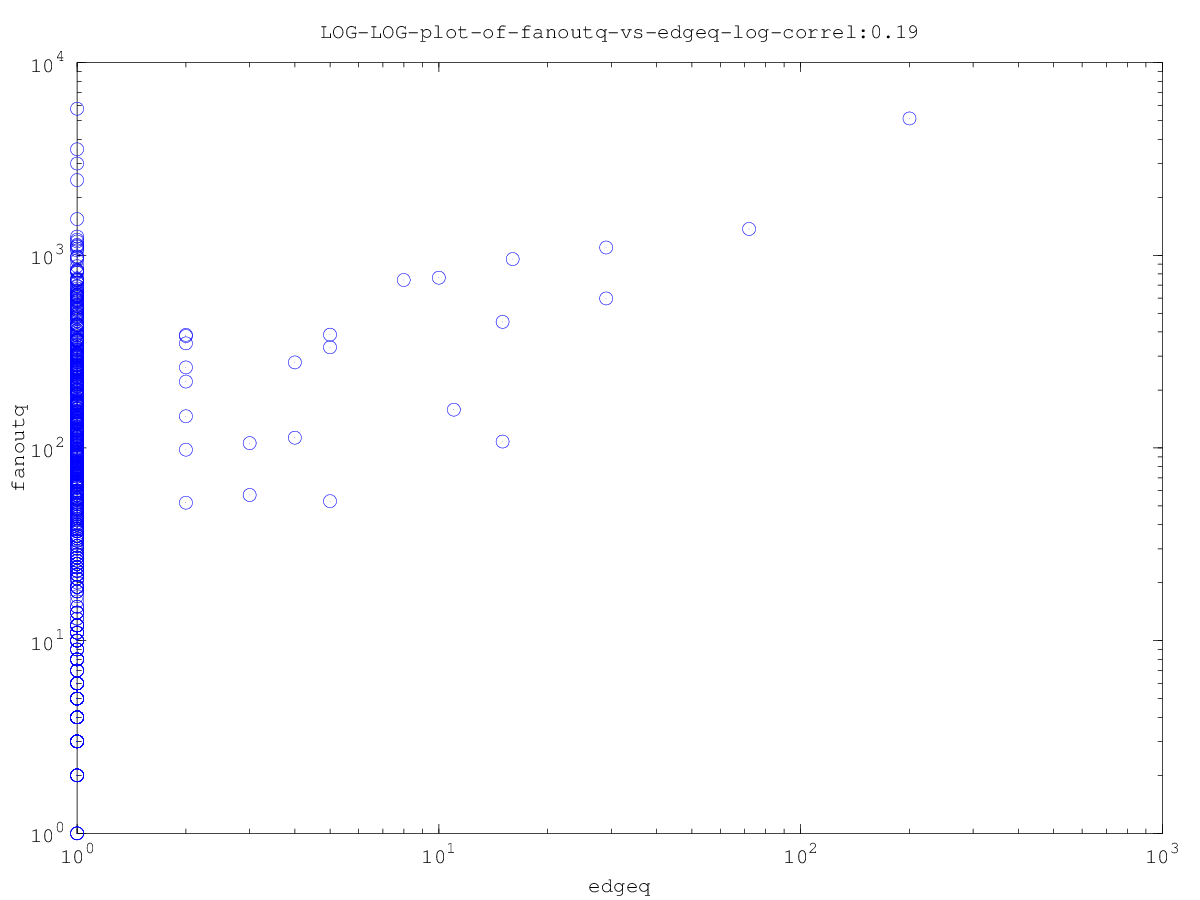
\includegraphics[width=\gridscale]{figures/LOG-LOG-plot-of-fanoutq-vs-edgeq-log-correl019.png}}\\
 \subfigure{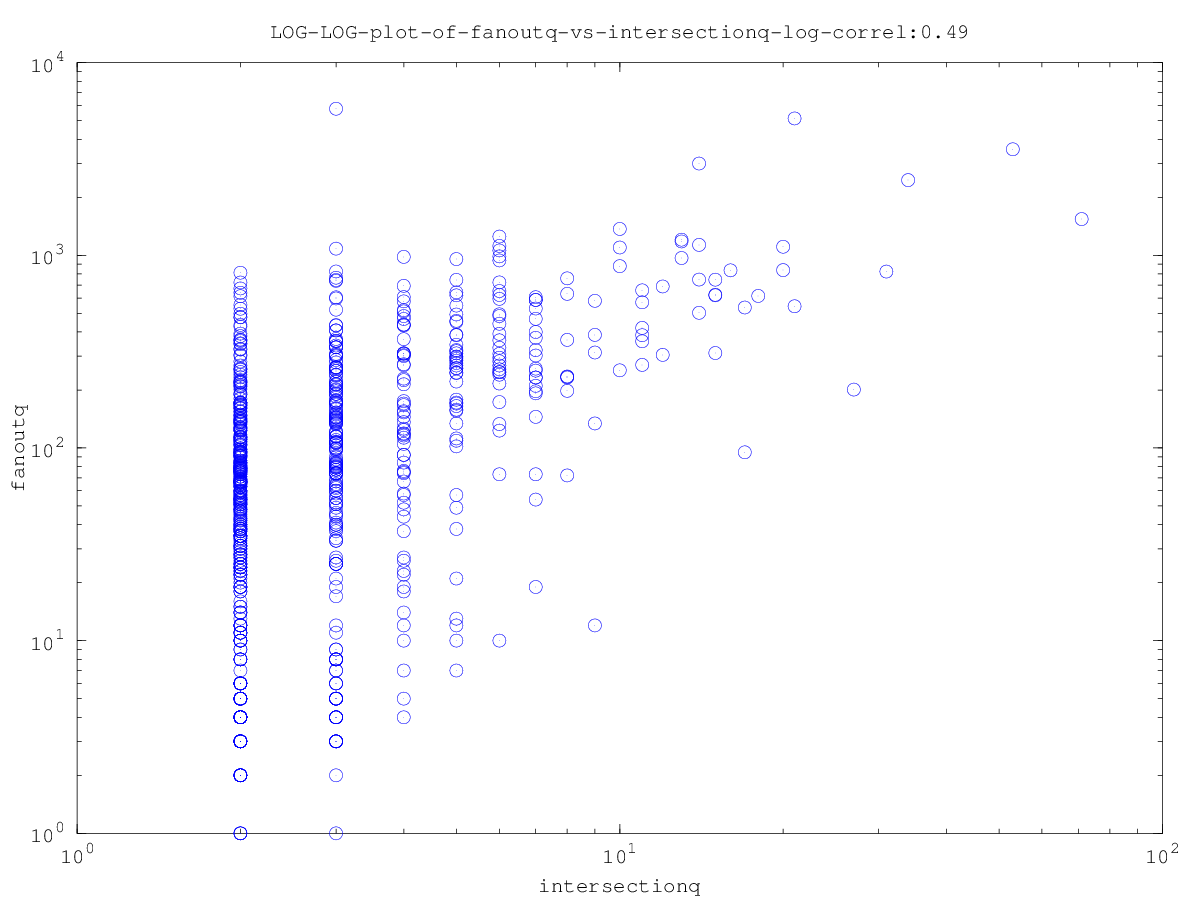
\includegraphics[width=\gridscale]{figures/LOG-LOG-plot-of-fanoutq-vs-intersectionq-log-correl049.png}}\\
 \subfigure{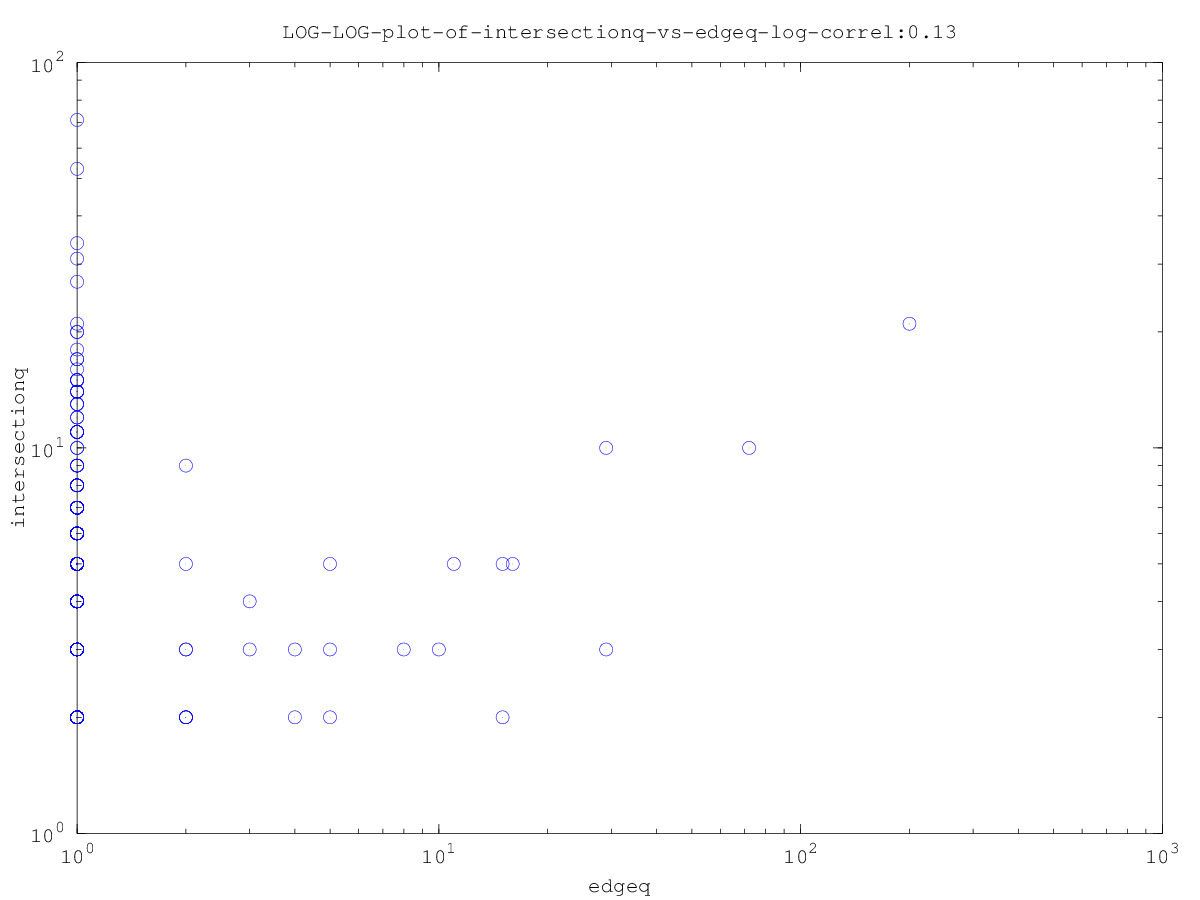
\includegraphics[width=\gridscale]{figures/LOG-LOG-plot-of-intersectionq-vs-edgeq-log-correl013.png}}
\caption{log-log scatterplots of correlations between query types}
\label{fig:querycorr}
\end{figure}

The edge metadata queries happen much less often, so the scatter plot has many points on the zero line (in the log sample). Also, these plots are made on a log-log scale, because they appear somewhat uniform, it implies some users get orders of magnitude more queries than others.   Interestingly, fanout queries and intersection queries are visibly correlated. Edge queries are not not as much. If we remove the nodes that have no edge queries at all, on the other hand, x

\subsection{Data}

As of September 2011 Twitter had an active user population of 100 Million \cite{twitter}.  The total graph stored can only be larger, as it contains all users from all time as well. The total number of edges between these active users is more than an order of magnitude above that, if we assume between 10 and 100 followers per user on average.   For the benchmarks run (described in section \ref{section:benchreal}) I worked with an older snapshot of the graph with 130 million (active and non-active) vertices and an average follower count of 40, for a total of about 5 billion directed edges. For these particular measurements I used a sample of this data set joined with the  sampled query logs of Section \ref{section:workload}.

Like with many other naturally occurring graphs, the degree distribution is similar to a power law: most of the users have relatively small degree (less than 100) but with a still substantial tail of users having larger degrees (the heaviest users have more than 10 million) and the decay behaving like the curve $1/x^2$. The maximum degree was 1 million.  The relation between in-degree (followers) and out-degree (people followed by user) is shown in Figure~\ref{fig:degcorr}.

\begin{figure}
\centering
   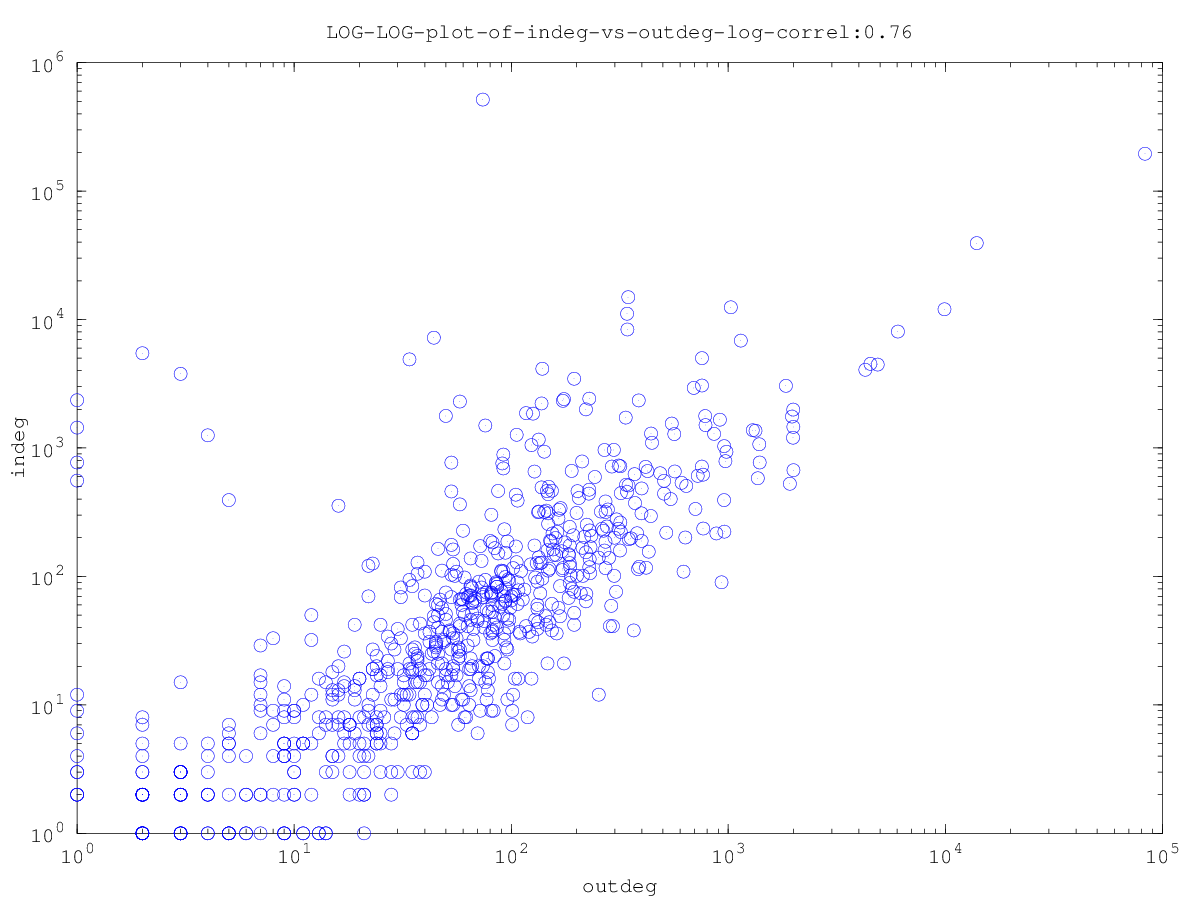
\includegraphics[width=\gridscale]{figures/LOG-LOG-plot-of-indeg-vs-outdeg-log-correl076.png}
   \caption{log-log scatter plot of in-degree vs out-degree}
   \label{fig:degcorr}
\end{figure}


%% %% LOG-LOG-plot-of-fanoutq-vs-edgeq-log-correl019.png          LOG-LOG-plot-of-indeg-vs-outdeg-log-correl076.png
%% %% LOG-LOG-plot-of-fanoutq-vs-intersectionq-log-correl049.png  LOG-LOG-plot-of-intersectionq-vs-edgeq-log-correl013.png
%% %% LOG-LOG-plot-of-indeg-vs-edgeq-log-correl002.png            LOG-LOG-plot-of-outdeg-vs-edgeq-log-correl004.png
%% %% LOG-LOG-plot-of-indeg-vs-fanoutq-log-correl001.png          LOG-LOG-plot-of-outdeg-vs-fanoutq-log-correl006.png
%% %% LOG-LOG-plot-of-outdeg-vs-intersectionq-log-correl009.png

From the figure we can again tell both the out-degree and in-degree distributions (for this small sample) already spans a few orders of magnitude. The in-degree (number of followers) is more spread out than the out-degree (number of people user follows), but they are highly correlated.  One consequence of this is that it may make sense to store the out edges separately from the in edges for heavy weight users at least.

One last measurement of interest is checking for correlations between user degree and workload. In other words, are you queried more if you have more followers or is there no correlation? The possibility of correlation would have implications. If large users were queried less often than smaller users, then optimizing for them is less important. If they are queried very often, relative to smaller users, then they are more significant to the performance metrics. There are arguments why this could happen: perhaps heavy users are much more involved in their accounts, or tweet more often.  Also, nodes with very large degrees imply a write for each of their edges.     By joining the log records from section \ref{section:workload} with the graph snapshot  used, we checked if wthere were any significant trends. The results are shown in Figure~\ref{fig:degworkload}.

\begin{figure}
\centering

  \subfigure{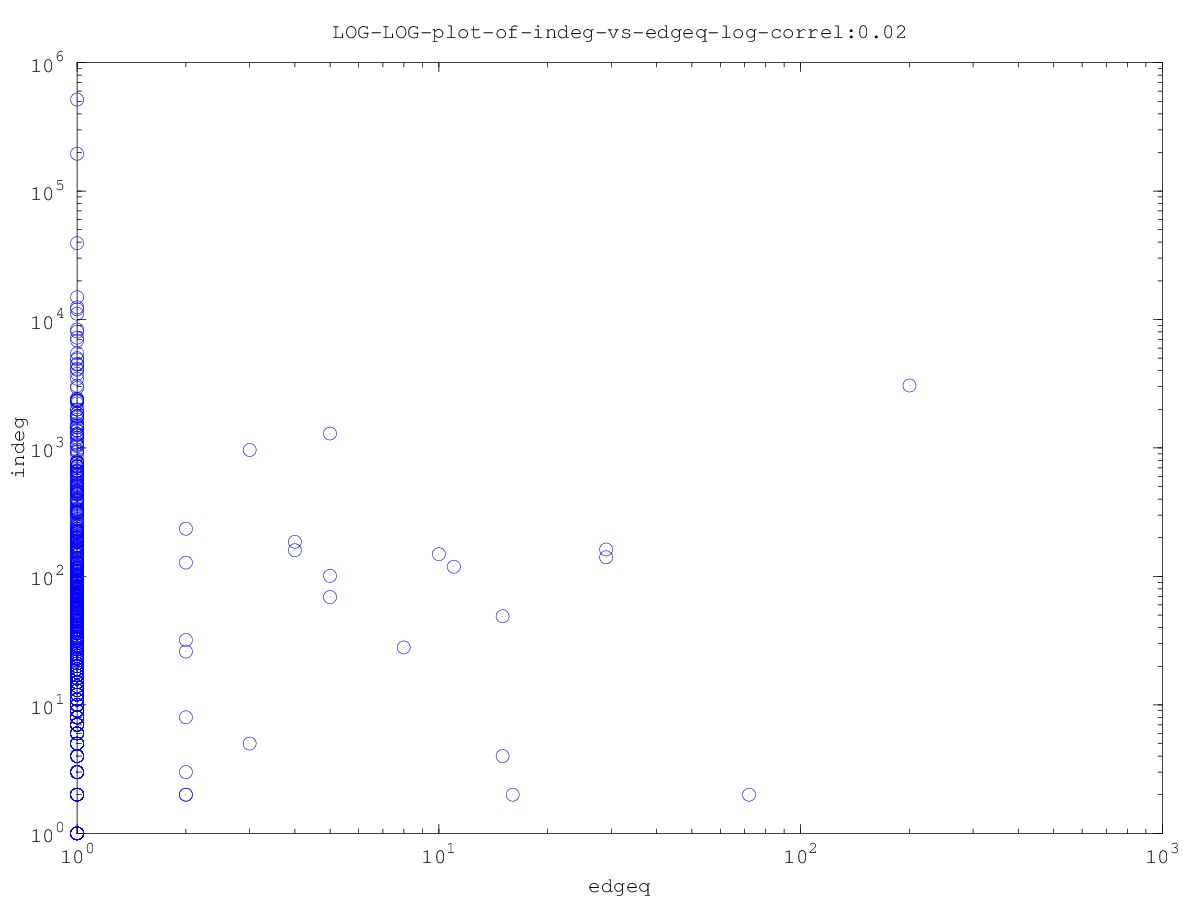
\includegraphics[width=3.5in]{figures/LOG-LOG-plot-of-indeg-vs-edgeq-log-correl002.png}} \\
  \subfigure{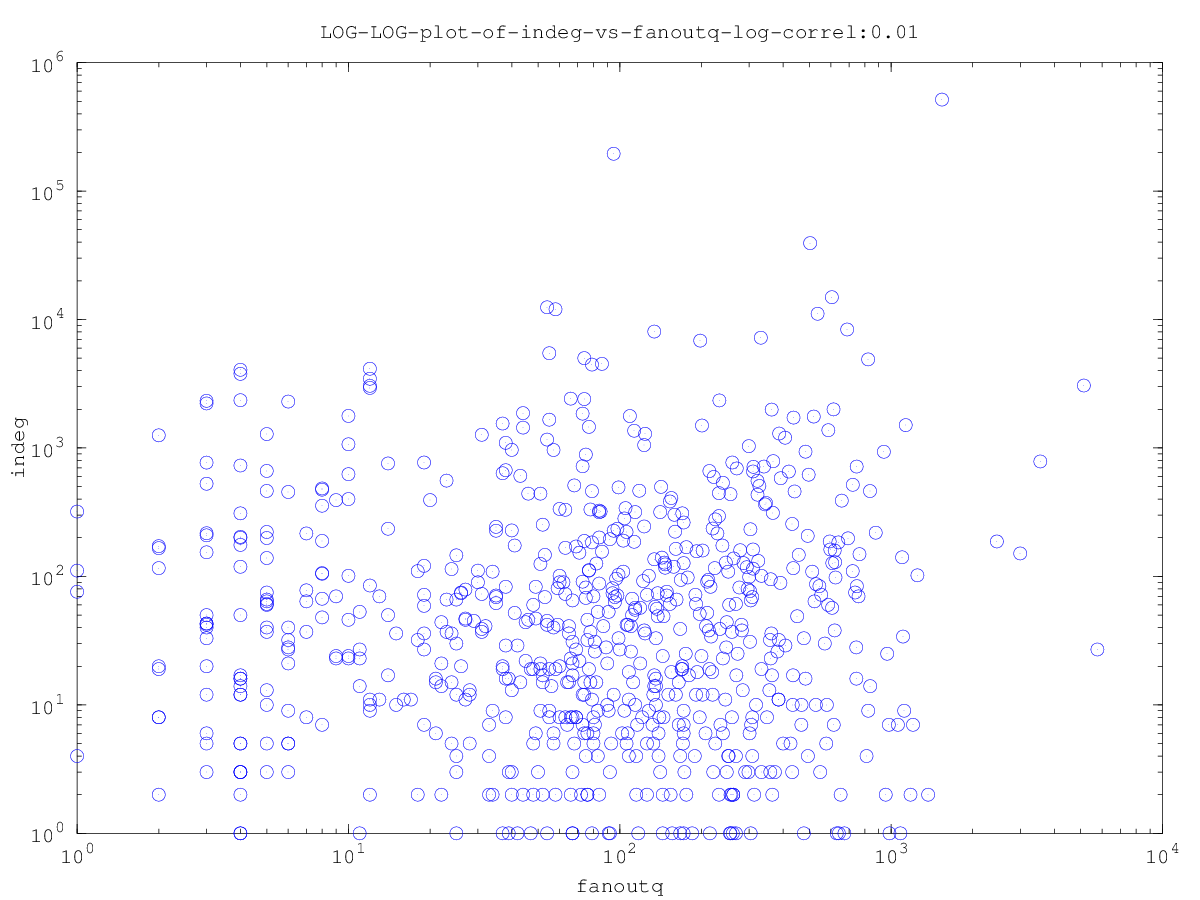
\includegraphics[width=3.5in]{figures/LOG-LOG-plot-of-indeg-vs-fanoutq-log-correl001.png}}\\
  \subfigure{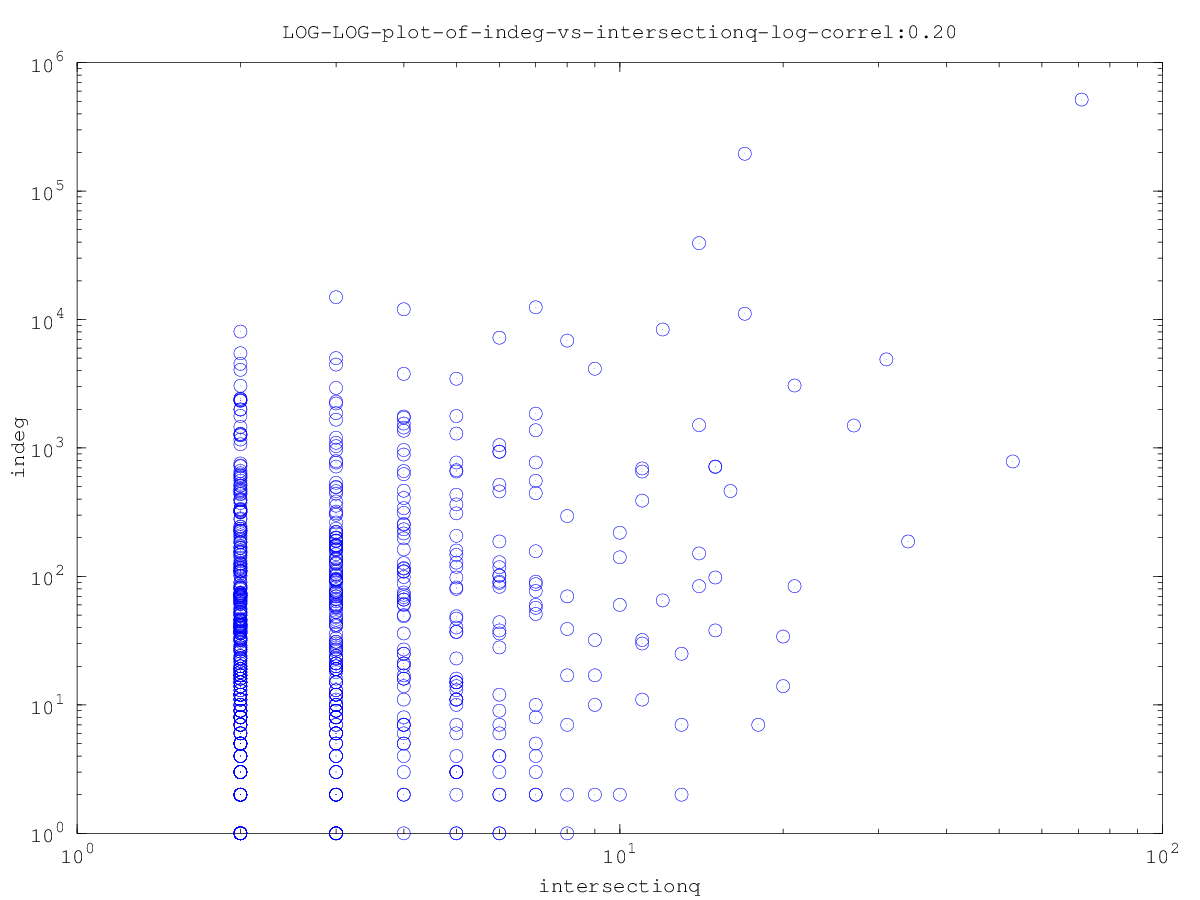
\includegraphics[width=3.5in]{figures/LOG-LOG-plot-of-indeg-vs-intersectionq-log-correl020.png}}\\

\caption{correlations between query popularity and number of followers}
\label{fig:degworkload}

\end{figure}

Edge and fanout queries show little correlaton with in-degree (number of followers), but intersections do show a postive relation.  Out degree (number of people followed by user) relates less strongly with intersection queries.

\chapter{Optimizing fanout queries}

While we are focused mostly on the performance of reading queries, writes are one of the graph database's main purposes (as opposed to the more analytical types of systems).  Also, the kinds of techniques considered do not aim to improve reads at the cost of writes. So we do not  techniques that make writing more expensive.

\section{Optimizing fanout queries with two tier hashing}
\label{section:optfanout}
The main original contribution in this thesis is the idea, that for fanoutq queries, it pays to treat heavy degree vertices different from light degree ones.  There are two factors in play here, one is,  

1) in general, the system users benefit from reducing the variance in latency across calls (which reflects an underlying variance in degree) by making it more predictable. 

% we are talking about latency for a single operation (not for latency of several ones)

2) some latencies are simply too large to be acceptable %copy back of the envelope showing this
and the problem will keep getting worse.  An important feature of a service like twitter is the real-time feel it gives its users. It is undesirable to  becomes notable that some users receive tweets much before others. This also implies more complicated design within the rest of the system, as application logic demands no user sees a reply to a tweet before receving the tweet first.  Hence, extra work is done at different layers to hold on to tweets that cannot be delivered yet, 

This property is present in many naturally arising relations. eg. social networks etc.

This feature comes at the cost of complexity in the sharding mechanism. In fact, since there is no relation between the user id and whether it has a large degree, it is necessary to introduce lookup tables for this purpose. Luckily, we can use the graph property that  the degree is very skewed against itself: we only need to remember very few. 

%todo add another back of the envelope

This condition is helpful it would not be less plausible with a graph where there are two equally large classes of nodes to have a table for half those cases. in that case, though, we can do something such as cacheing, in case access patterns show some kind of skew. %complexity problems related to look

%(actually it would be interesting to analyze how cacheing relates to this, and maybe propose a solution based on it. Cacheing depends on skewedness in access patterns (ie acesess are only like to a few places), but cacheing policies can normally adapt online to handle distributions that change over time, as long as they remain skewed. Also, cacheing when the requests have a fanout.

For a given fanout size, there is an optimal number of partitions with respect to latency. For throughput, the optimal is probably  closer to 1.


The two main factors potentially afecting latency are 1) variability in network communication: the more nodes we request data from, the more likely
at least one will lag, affecting the performance of the whole operation 2) the more nodes we have, the more parallelism there is in reading.

\subsection{The cost of parallel requests}
Whenever we parallelize calls we reduce the work done at each node, but add the overhead of making more calls. If the calls are all made in a sequence (but without waiting for the previous to return in order to start the next), then we still have a cost linear in the number of nodes involved, with a smaller constant.    This overhead can be controlled by making a tree of calls (where a the calls themselves are organized in parallel), reducing this overhead to a $\lg{n}$ factor.  Nevertheless, there is an extra cost to making more calls. Each call made over a network has a natural, random, variability in latency. Since ultimately we need to wait for each of the parallel calls to finish, then we need to wait for the worst case of $n$. As $n$ increases, the latencies at each percentile level increase also. The exact way in which they increase depends on the original distribution.

For example, if we assume the latency of a single request is exponentially distributed, and that each request's latency is identically distributed but independent of the others done in parallel, as we increase the number of nodes we get the trends in figure~\ref{fig:fanout_effect}


\begin{figure}
\includegraphics[scale=0.25]{figures/exponential_latency.png}\\
\includegraphics[scale=0.25]{figures/powerlaw_s2_latency.png}\\
\includegraphics[scale=0.25]{figures/uniform_dist_latency.png}
\label{fig:fanout_effect}
\end{figure}

The other two figures show the same  trends: at a fixed percentile, latency is monotonic on  the number of participating nodes. In a cluster with 100 machines or more, this can have a significant effect in latency. The data for these graphs is based on simulation, simply generates a random value for each of the parallel requests and takes the maximum, many times. 

Also importantly, the exact relation between fanout size and latency due to variability can be linear, sublinear or super linear depending on the distribution. For A bounded distribution, for example the latency quickly devolves to the worst case scenario. This illuminates interesting implications, for example in a systemw with n paralley systems each of which may hit or miss in a cache with probability p, fixed. If the chances of hitting the cache are independent, the effectivness of cacheing drops as we increase fanout. On the other hand, cache hits are likely to be dependent so perhaps this is not as practially relevant. On the other hand, network latency itself may be more independent. Similar effects are a consideration in RAID systems, together with increased parallelism  we have the an increased expected cost of seek. For one disk, we expect a seek to take about half a disk revolution. As we add more disks, it is more and more likely at least one of them will go around a full revolution, forcing everyone else to wait that same amount.

Some authors have also explored the effects of increased fanout on service latency [ref google latency slides]. The previous figures show that it is correct to assume an increased latency. For our analysis, we will assume a linear cost (consistent with some kinds of latency variability). 

These factors can be expressed as \(L = max_{i=1}^n(L_i) + q*d/n\), \(q\) is a system specific constant, \(d\) stands for a fixed degree, so we are splitting the fanout into many and the latencies \(L_i\) are random, with some distribution (eg exponential). Presumably the \(f(n) = E[max_{i=1}^n(L_i)]\)  is an increasing function of \(n\). so \(E[L]  = E[max_{i=1}^n(L_i)] + work/n\). DeWitt etal  model this by  assuming \(L = kn\) for some system specific constant \(k\).  With that assumption, optimizing \(n\) to minimize latency is straightforward: 

\[ L = kn + qd/n \]
\[ dL/dn = k - qd/n^2 \]
\[ n_{opt}(d) =  \sqrt{qd/k} \]
\[ L_{min}(d) =  2\sqrt{qkd} \]

In a system where there is no cost associated with increased parallelism the `minimum' latency  would be (close to) zero, as we could simply increase $n$ arbitrarily.
The minimum latency achievable depends both on the degree itself, and on the other system parameters.

So when we partition every vertex optimally depending on its degree, latency grows as $\Theta (\sqrt{d})$, whereas with a naive hash by vertex approach, latency grows as $\Theta (d)$.  This formula is not completely faithful to reality, because actually $n$ and $d$ are restricted to postive integers, so $2\sqrt{qdn}$ would suggest the minimum work needed when $d=1$ and $n=1$ is $2\sqrt{qk}$, when in actuality it is $q + k$..

If we choose a cutoff $t$ so that

If $d < t$ we do plain vertex sharding, and if $d > t$ we behave optimally, 
then we get
% can show plot shape.

Think about per-edge latency. Is it importat? Eg. for a fanout per edge latency tells you how much time it took a  followers to have a tweet delivered.

The above analysis was valid for a particular \(d\) variable. So this would be the optimal partitioning for vertices of a particular degree.  Where there is variation of degrees, in the best possible world we would treat each node according to its degree. A sharding function would need to figure out based on the node how to treat it, so we would need a lookup table for that. This would be unrealistic (right?). unless we keep a table of size O(number of nodes).

Alternatively, it is feasible to degrade the granularity, and pick a threshold \(B\) such that we  divide all nodes with \(deg > B\) one way, and the rest another.

Given a B, We can optimize differently for each part (and also, we can further optimize for the B) and implement this by remembering only the nodes above the threshold. This way we get a much smaller lookup table.  Optimizing for each of these independently brings together many strategies that may seem very different if treated in isolation (such as shard everyone into 2 parts no matter the degree,  or  for degrees above 10k,  shard into all machines) and picks the best.

(this more careful analysis still needs to be done)

Potential problems are how the optimal changes as the graph grows.

%todo. Analysis of added problems of sharding mechanism in dynamic situation.

\subsection{Experiments on synthetic data}
To test the different strategies I constructed a basic system consisting of query router server and  several data notes in the backend.  The query backend server 

Designed a benchmark with skew on ID queried, but iid. Designed a way of generating graphs for querying fanouts (random degree). The benchmark allows me to control 
query skew, while the graph allows me to control degree skew, or a constant degree.

The argument about skewed degrees and lookup tables implies that the more skewed a degree is, the easier it is to implement lookup tables. while also the less relevant it is
(because having only 1 large user and 1 million small ones means it might be acceptable to degrade. On the other hand, if skew is 1, then actually 'work' graph is very uniform.and if the parameter is less than 1, the work is actually all concentrated at the top!, so arguably you should design for it.

ie. let  \(D\) be the random variable representing the degree of a randomly picked vertex. Assume \(D\) has a distribution \(p_D(n) 1/n^\alpha \) then let \(E \) be the degree of an edge, where we define the degree of an edge to be the number of other edges in the same node. (directed? or sum?). \(p_D \) and  \(p_E \) are related in the following way:

\( p_E(n) = n*p_D(n)\). This relation expresses that in a graph with vertices of varied degree, edges are more likely to be around large degree nodes. 

 is making cases where \(n \) is large more likely. 

Caveat: cacheing and size control. How can we 1) increase the degree of every node 2) keep total database size constant 3) not increase locality.
I gave up on keeping database size constant, so some database were more full than others. To avoid cache effects. (not even sure if i controlled this effect well)


To test this method more thoroughly, I generated a syntehtic graph with about 1000 vertices,  with degrees ranging from 1 edge to 10 million, and a skew parameter of 1. (Twitter's graph store has a similar range of values, though a lot more vertices).  I ran a benchmark of pure fanout requests for vertices chosen uniformly at random from the 1000, under three different strategies: a simple hash by vertex, a two-tier hash, and an all shards, on a cluster of 13 computers.

We expect the two-tier and all shards to do well at the higher percentiles, and the two-tier and vertex strateges to do better at the lower percentiles, showing the benefits of the fine grained approach.  This is what figure  \ref{fig:skew1_n13}  shows. The median latency of all three strategies 988musec  for all shards, 549musec for twotier and 748 musec for single shard show all shards increaes the median latency. Lower latency percentiles show more strikingly how all shards queries are expensive. the 10\% fastest requests ran in  up to 850 musec for all shards whereas in the two-tier case this was 348 musec, and 590 for the single vertex hash.  At the 90th percentile, all-shards queries and two-tier take 2653musec and 2605musec respectively,   whereas the single shard takes a substationally longer 9938 musec and improvement of more than 50\%. As expected, This improvement is even higher at the 99th percentile: all-shards and two-tier each take about 9000 musec, whereas single vertex took 76000musec.

\begin{figure}
%% n13.d1-10m.q100k.v1k.all_shards_histogram_newdata-2012-04-23T20.44.36.426.log.png  
%% n13.d1-10m.s=1.q100k.v1k_VERTEX_histogram_newdata-2012-04-23T21.10.08.869.log.png
%% n13.d1-10m.q100k.v1k.two_tier_histogram_newdata-2012-04-23T21.23.01.252.log.png    
\includegraphics[scale=0.25]{figures/VERTEXs1.png}\\
\includegraphics[scale=0.25]{figures/TWOTIERs1.png}\\
\includegraphics[scale=0.25]{figures/ALLSHARDSs1.png}
\label{fig:skew1_n13}
\end{figure}


The relative improvement from using the TWOTIER strategy depends both on tuning it and on the skew of the data.  Here the skew parameter was 1. If we increase it to 1.1 (ie decrease the number of extremely heavy nodes).  The larger the chances of extreme cases, the better a two-tier strategy performs relative to either strategy at all latency percentile ranges. 

\subsection{Experiments on real data}

Ran it with a threshold at ??(top 1m) into 5 parts, rest .  Latency behaved as follows:

The bad news are I arrived at this setting through tuning a program that was not well optimized, after I optimized it.

\begin{figure}
  \begin{center}
      \scalebox{0.25}{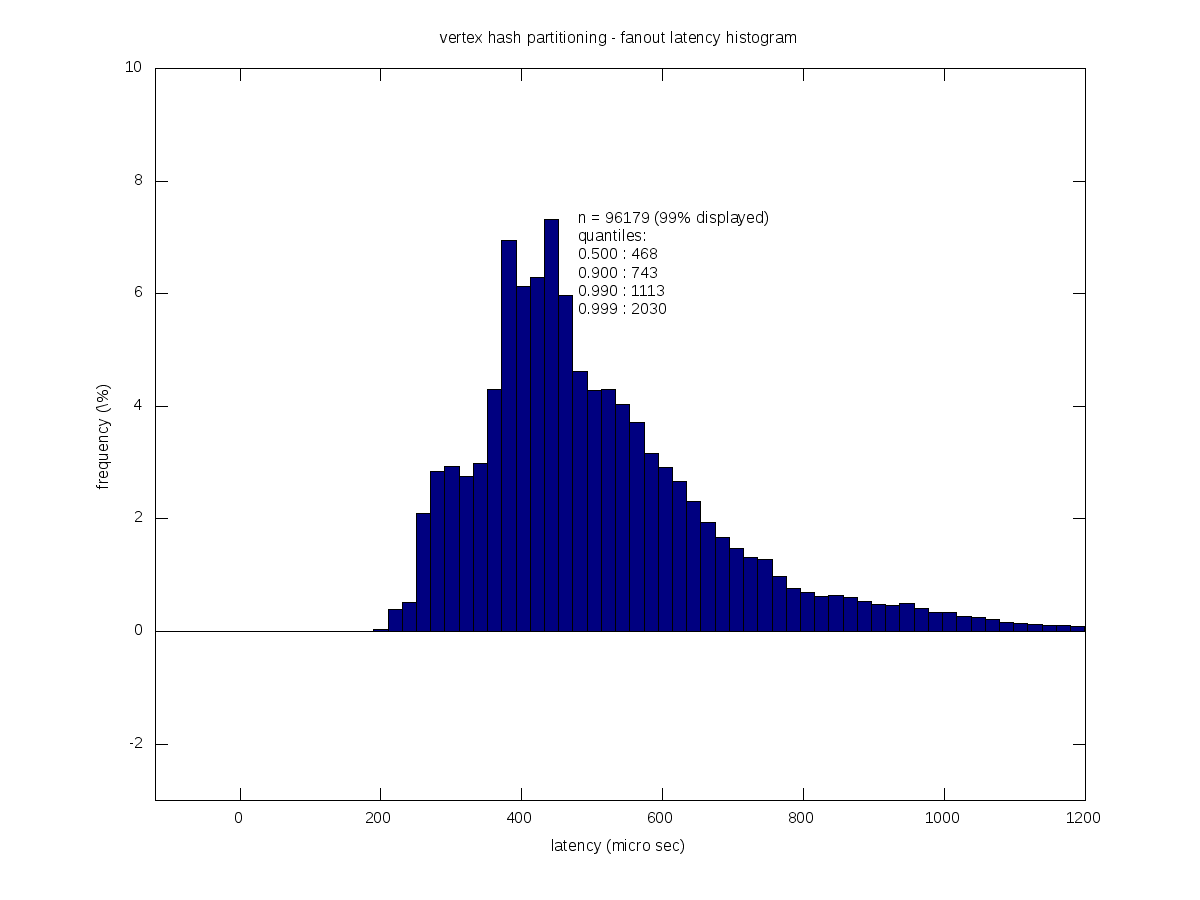
\includegraphics{figures/vertex-fanout.png}}
      \scalebox{0.25}{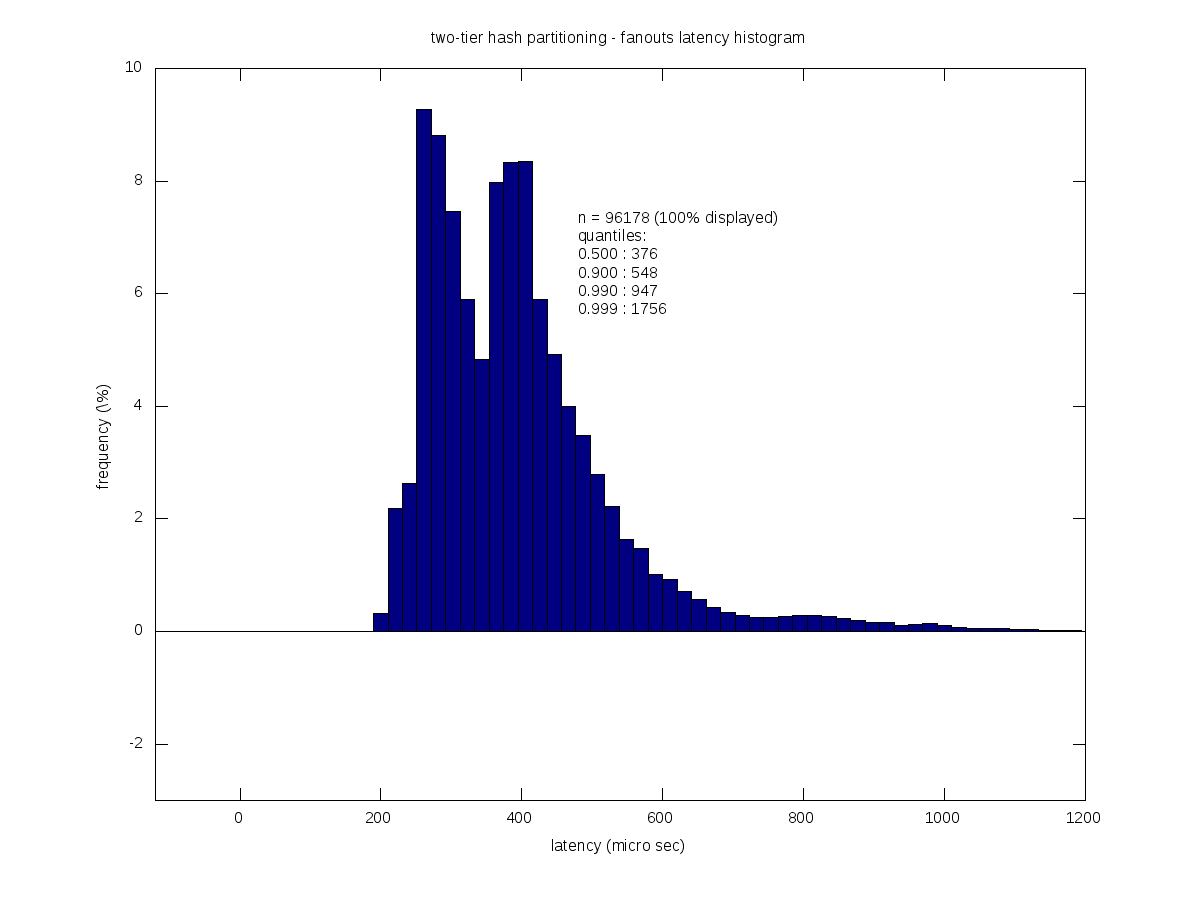
\includegraphics{figures/two-tier2m-fanouts.png}}
      \scalebox{0.25}{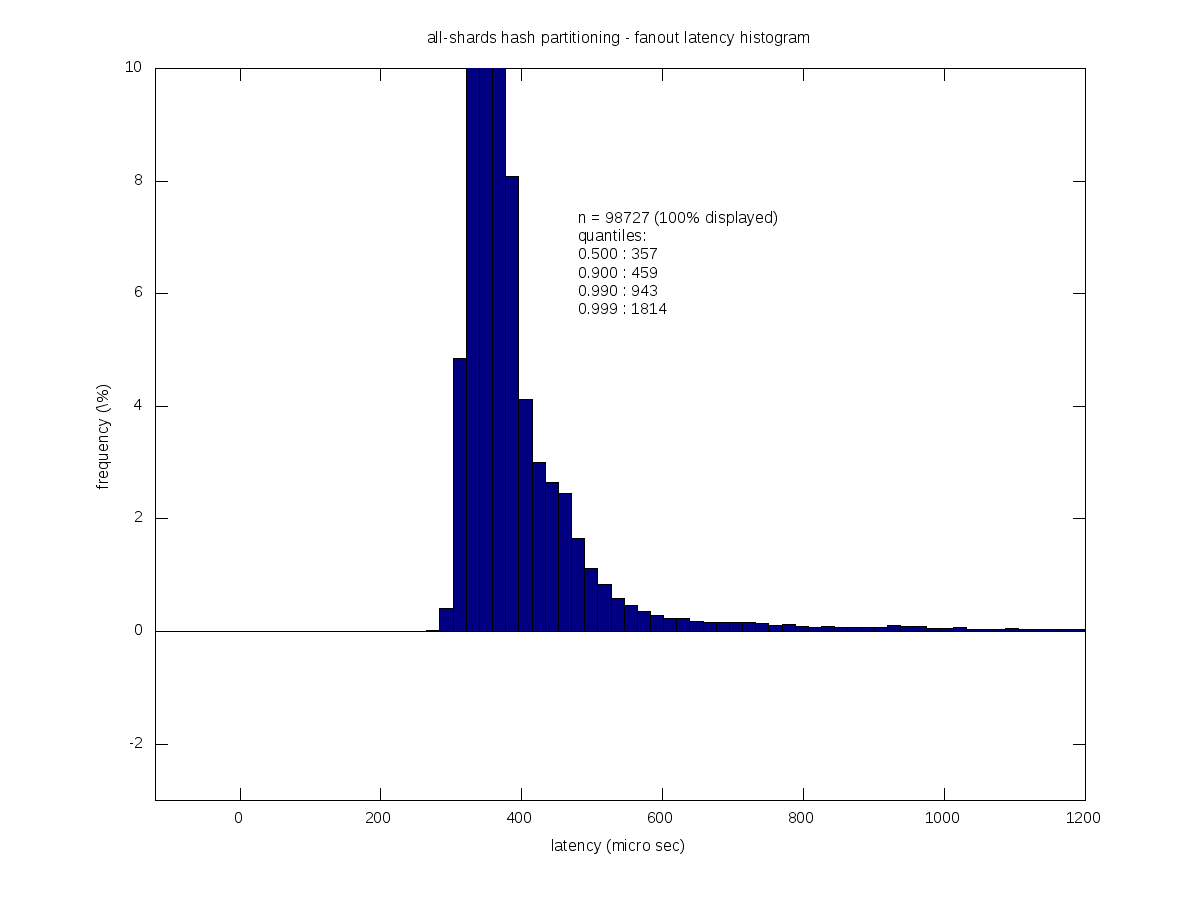
\includegraphics{figures/all-shards-fanout.png}}
  \end{center}
  \caption{Fanout latencies for a) vertex b) upper 2M tier c) all 5 shards hash}
  \label{fig:fanout}

\end{figure}

So when I checked to see performance for 5 way partitioning everything, I got even more improvements for the higher latency ranges. Note latency at higher percentiles is reduced, but increased at lower ones. 


%we never talked about measuring at the 99% percent level .

%percentile05.png  percentile10.png  percentile50.png  percentile99.png for plots of this trend.

\chapter{Optimizing intersection queries}

One motivation for allowing intersections and difference queries to the database is to push filtering as closde to the data as possible. Taking this one step further,  we prefer a query that gets resolved at a single node rather than involve an extra round of communication and external filtering.
I n chapter \ref{chap:background} we described systems that attempt to partition graphs based on its strucure, as well as work such as Schism \cite{schism} that accomplishes this. Ther are two aspects to improving intersection queries. The first is purely algorithmic. We can think of an intersectoin as an equijoin operation, and similar algorithms apply to both. In a distributed data base we attempt to partition tables equally on their frequently joined columns.  This allows easy parallelization of the query: first join locally.  

The optimal algorithm for intersection depends on the relative sizes of the two tables columns. In the case of the graph store, we can think of several possibilities:

%n * m,  n *log m, n logn +  m log m + n + m, n + m O(m) space
%may want to think a bit more about this?
\begin{enumerate}
\item nested loops: $O(nm)$ time, no extra space needed, only small constants costs.
\item sort the entried of the smaller one and then binary search for matches: $O((m + n)\lg{(m)})$ $m$ is the smaller one.
\item construct a hash representation of the smaller set and then query for matches: $O(m + n)$ time, $O(m)$ space, larger constants for constructing the hash.
\item sort- merge: $O(m \lg{m} + n \lg{n})$. If they are already sorted, then we only pay for the  $O(m + n)$ merge.
\end{enumerate}

There are other aspects about this that are important. Like with fanout queries, intersection queries are paged and may not require the full intersection set. They also may require the results in a particular attribute order (different from that of the id set). Moreover, whenever the two fanout sets to intersect are not in the same physical machine, we have to decide which of the two sets moves. 

One effect of limiting the size of the desired result is that the optimal plan may change. If we wish to only get latest common follower, we may want to avoid constructing a full hash. And, especially if the smaller set is very small, we may want to simply loop. There are many optimization techniques that could decide on how to perform the intersection based on the sets involved, and pick a method from the different choices presented.

We are focusing on the relation between partitioning and performance, so we don't try to find  the optimal intersection strategies but instead focus on the effect of reducing the number of distributed queries needed. The main idea we use for optimizing queries is that, just like Schism does for distributed transactions, distributed queries can be improved by using a workload driven approach. If we keep track of frequently intersected pairs and place them together, queries should take less time and the cluster should have a larger maximum throughput, as we consume less resources per query. In the background section we showed that some ids are  intersected a lot more often than others, so, like with fanouts, we

\subsection{Workload driven partitioning}
Imitating the steps from Schism, we partition the graph so that often intersected pairs get placed together. It is tempting for anyone thinking about this problem, including us initially to figure out a way of splitting the social graph  so as to place adjacent nodes together. This kind of partitioning seems natural, since the graph is social it is plausible to infer we should split it via communities  defined by this social structure.  This social graph driven approach has two drawbacks in the case of Twitter infrastructre. The first is the challenge of partitioning the full graph. In the offline case, the graph snapshot was heavy enough that we were not able to get a good result after running METIS for several hours, perhaps using the distributed alternative would speed things up (or maybe not, considering the added communicaton), or perhaps using one of the online algorithms available for this task could make it practical, but either way, the straight forward  approach did not seem to easily scale.   

The second reason this approach is not ideal is that they payoff for such a clustering is not clear either. In the case of Twitter, the user tweet tables  and the user tables are stored separately. Storing a user in the same machine as its followers does not imply more locality in intersection queries unless there is a strong correlation between being followers and intersections.  Since there are no other queries that need locality of this sort, we can avoid using any proxies and use the workload logs themselves to compute which intersections actually happen often.  This is the idea behind the workload driven partitioning. Ideally, this would be an online repartitioning algorithm.  In order to measure its potential effectiveness, on the other hand, I followed the approach suggested in the Schism paper \cite{schism}, and computed a partitioning offline using METIS. The difference is that instead of the social graph driven approach, the graph partitioined by metis is the `operation' graph of a sample. 

We define the operation graph as follows: 

\newtheorem{definition}{Definition}
\begin{definition}
  Follows graph.
  
  Directed graph $G = (V,E)$ where the $V$ are users and an edge $(v,w)$ is in $E$ if and only if $v$ follows $w$.
\end{definition}

\begin{definition}
  Workload graph (for a time interval) 

  Symmetric weighted graph $W_G = (V',E')$  with $V'$ a subset of $V$, with vertex weight for $v$ proportional number of queries involving $v$ in the given interval,  and with edges $\{v, w\}$ in $E'$ with weight $\omega_{vw}$ proportional to the number of intersections involving $v$ and $w$ in the same time interval.
\end{definition}

Both the follows graph $G$  and the corresponding workload graph $W_G$  change over time as edges and vertices are added, but  $W_G$ changes even if $G$ remains the same, depending on the queries received in that time interval.   There are important difference between these graphs. Partitioning $G$ evenly implies that the amount of data stored per node is balanced. Partitioning $G$ minimzing edges means a node is likely to be close to its followers.  On the other hand,  partitioning $W_G$ evenly implies that actual work done across the partitions is even, and that nodes that are often intersected are close together.   Other important differences are that $W_G$ can be small if the time interval is small enough, which provides us a natural way of sampling it by simply sampling the logs.  

In the case of the experiments in this thesis, from the sampled query logs we obtained a graph of 10 million edges (down from 5 billion inthe sampled follows graph). So the partitioning problem is much more tractable.  We did not investigate what the optimal size of the sample is, but this particular sample was enough to improve intersection performance.

(not so for the graph) mention sampling paper.
Importance of adaptive approaches: new stars rise in a matter of days to 
%find a place for this sentence
In effect, because they are different services we can think of the the data tables of users, follows, timelines as vertically partitioned.

% we can mention how the giraph developer argues disconnected nodes may talk to each other as well.
%here we can add synthetic experiment for throughput (but may need to implement descentralized intersections first)

\subsection{Experiments on real data}

We tested the workload driven partitioning strategy on the graph snapshot describe in \ref{chapter:twitterbackground}, using the query logs also described there and a few map-reduce jobs to generate the workload graph and METIS to partition it.  Since the query graph includes only a about 10\%  of the total nodes, we partition the rest of the graph using a hash function and similar to \ref{section:optfanout}.

We then replayed the same log traffic on a database loaded with the same snapshot as above,  One possible effect of this is that performance is better (since we are training on the same data set we are testing), but the experiment is still meaningful because the workload graph is only a proxy for the real workload. 

Results running the intersection queries (for the three techniques) are shown in \ref{fig:intersection}.

\begin{figure}
  \begin{center}
      \scalebox{0.25}{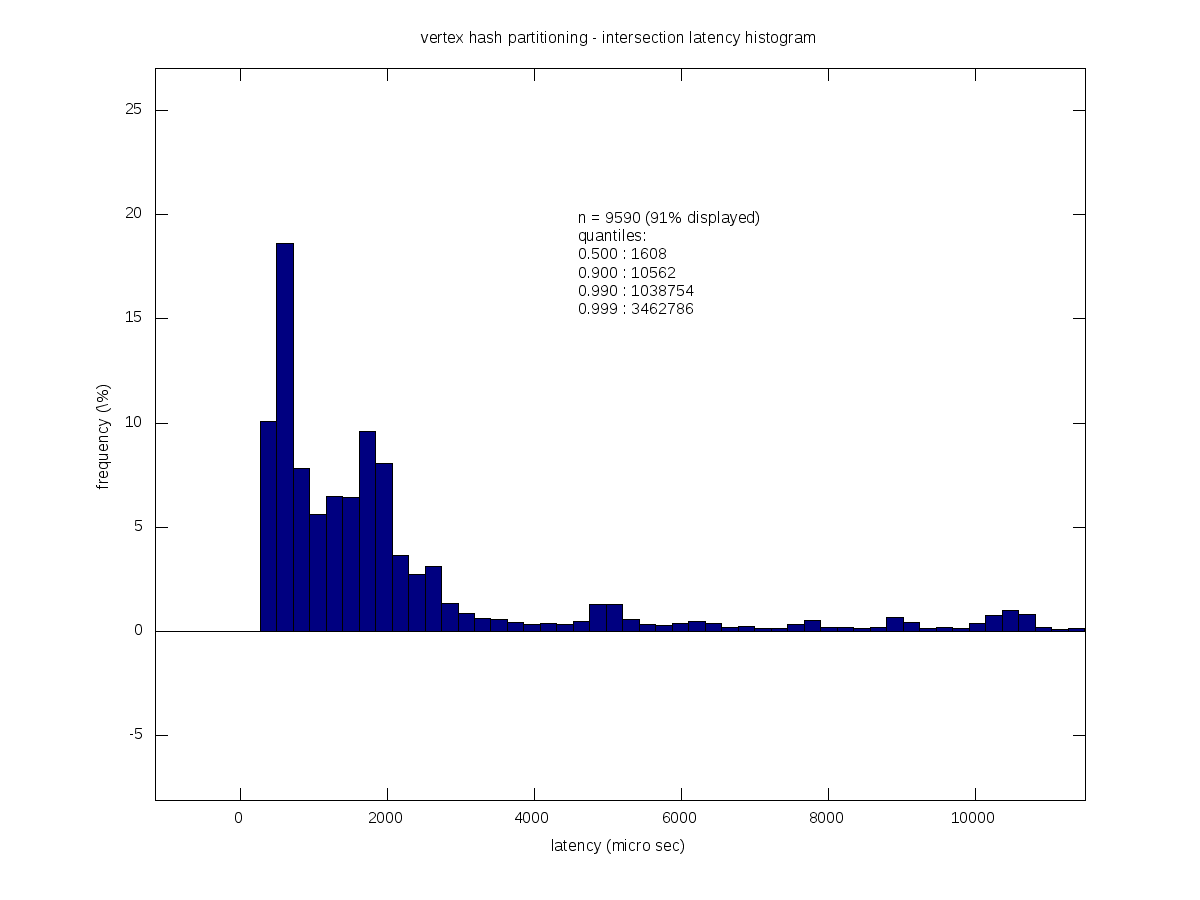
\includegraphics{figures/vertex-intersection.png}}
      \scalebox{0.25}{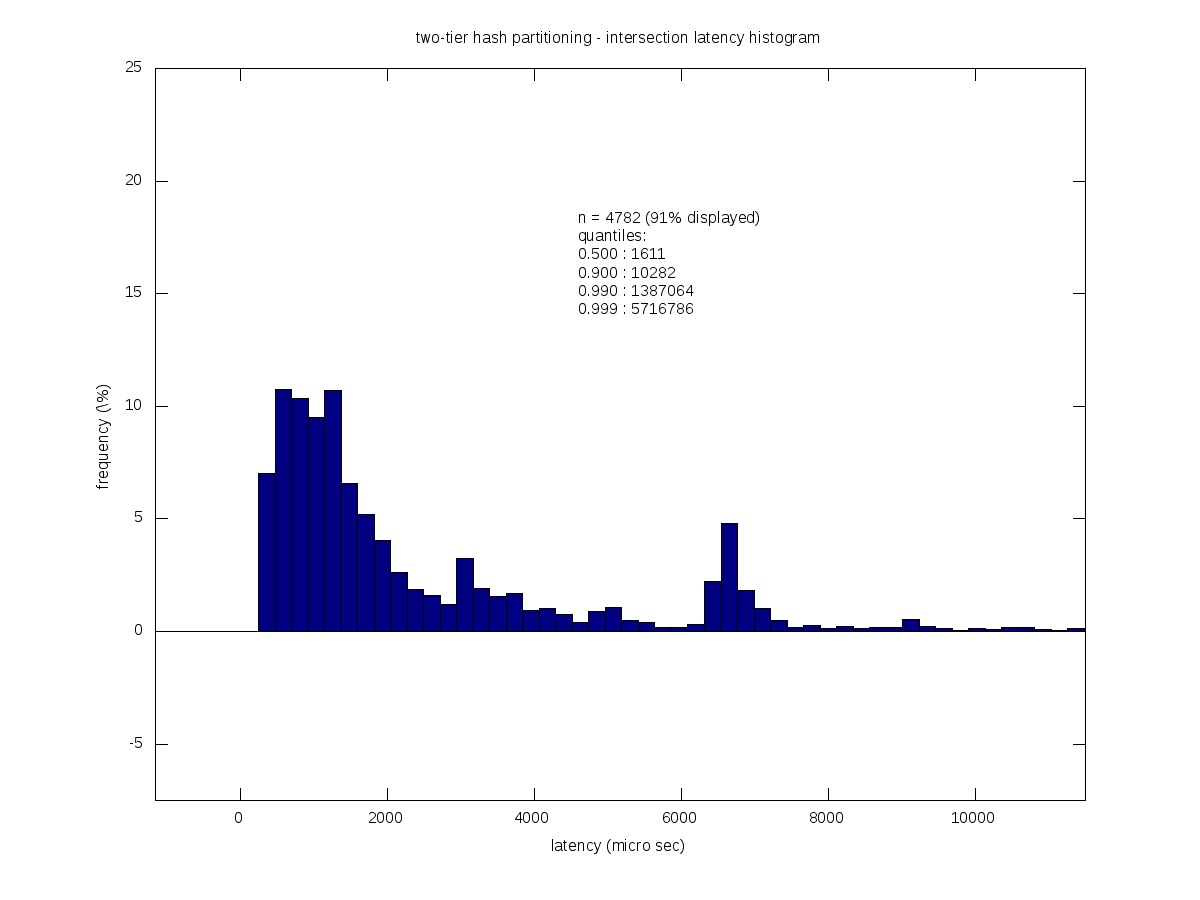
\includegraphics{figures/two-tier2m-intersection.png}}
      \scalebox{0.25}{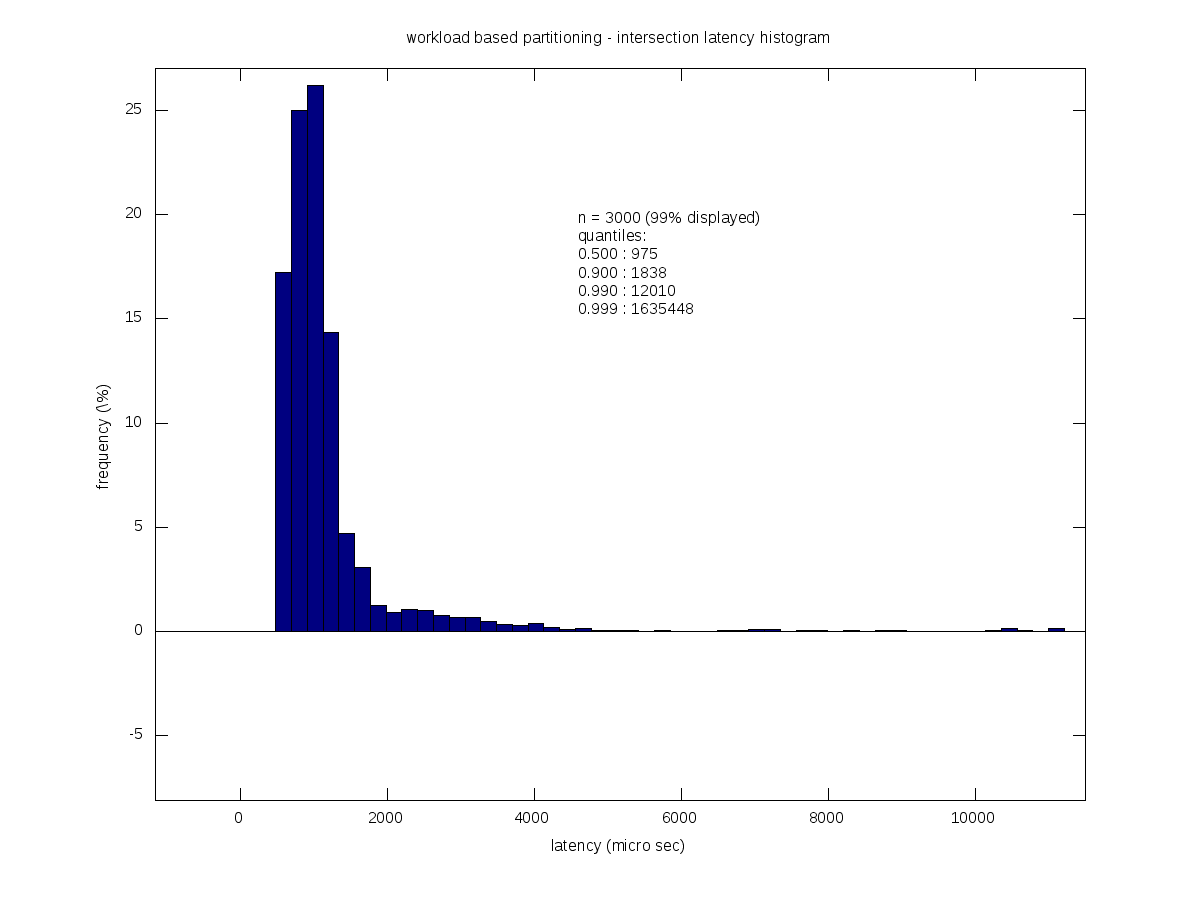
\includegraphics{figures/workload-intersection.png}}
  \end{center}
  \label{fig:intersection}
  \caption{Intersection latencies for a) vertex b) upper 2M tier c) workload based}
\end{figure}


\section{Design}
%information about what I built, (java and pig) goes here. information about results goes here too.

The system was implemented in Java, with a routing layer (the APIServer) that communicated with the data nodes based on its lookup tables via Java RMI calls. Each of the nodes were identical, and held the edge information in memory. For the purposes of this experiment I did not need to support persistence or concurrent modification of the data, since I was measuring read latencies.  I also did not need to support fully dynamic structures, which allowed me to fit enough data using sorted arrays rather than much more space hungry Java maps. These limitations are not fundamental though. Future generations of many Twitter services will be in memory, and disk would be used only to survive. For in memory databases it isn't that necessary to support concurrent writes, because there is no IO bottleneck to use parallelism against. Finally, in a real system the data can be stored compactly by using custom data structures that take much less space, and using systems implement in languages less memory hungry than Java.  Using sorted (static) arrays rather than binary search trees keeps the search time to $O(\lg{n})$. This is helpful to implement the offset logic. It also allows ordered scans of the fanouts that can be merged. Such ordered reads may be less realistic than in a B-tree since they have a lot more locality, but since we only aim to compare the difference between latency at different sizes, it is not a problem.

For benchmark generation I also improved on a ZipfGenerator, which turned out to be a bottleneck whenever I needed to generate numbers zipf distributed in a long interval. Memoization of frequently used internal values helped improve it by far.

The system used in testing the SPAR  heuristic distributes the directory itself into a Hash table.


\chapter{Related and future work}
%here I should bring in some of the background section, and show how it relates 

One interesting topic is analyzing way to make either partitioning adapt to a changing graph. In the case of two-tier hashing we need to react to a node gaining many followers  by repartitioning into several nodes. And, as the node gains more and more followers, keep repartitioning. One option is to use queries as a way to keep a count on followers. Then, use a technique such as consistent hashing to minimize the amount of data moved as we readjust.

For the workload graph based strategy, it is more complicated.  
online partitioning?a
correlation between actual graph and intersection graph?
Neo4j partitioning? how can they do it or do they avoid it? they did not support it at the beginning at least?





\section{Loose ends}
%measuring throughput behavior. Stuff like mixing both strategies, making the algorithms online. Talk about the way to implement this system so that it reacts to new stars well. 


\section{Conclusion}


%% \appendix
%% \include{appa}
%% \include{appb}
%% This defines the bibliography file (main.bib) and the bibliography style.
%% If you want to create a bibliography file by hand, change the contents of
%% this file to a `thebibliography' environment.  For more information 
%% see section 4.3 of the LaTeX manual.
\begin{singlespace}
\nocite{*}
\bibliography{bib/more,bib/metis}
\bibliographystyle{plain}
\end{singlespace}

\end{document}

